\RequirePackage[l2tabu,orthodox]{nag}
\documentclass{article}
\usepackage{amsthm}
\usepackage{amssymb}
\usepackage{mathtools}
\usepackage{minted}

\usepackage[colorlinks=true,pagebackref,hyperindex,citecolor=myblue,linkcolor=mygreen,urlcolor=mygreen]{hyperref}
\usepackage[top=1in, bottom=1in, left=1.25in, right=1.25in]{geometry}

\usepackage{amsmath}
\usepackage{amsfonts}
\usepackage{amssymb}

\usepackage{color}
\usepackage[dvipsnames]{xcolor}
%\definecolor{myblue}{rgb}{0.16, 0.32, 0.75}
\definecolor{myblue}{rgb}{0.0, 0.45, 0.73}
\definecolor{mygreen}{rgb}{0.05, 0.5, 0.06}

\usepackage{mathrsfs}
\usepackage[mathcal]{euscript}
\usepackage{mathtools}

\usepackage{enumitem}

\usepackage{float}
\usepackage[center]{caption}

%\usepackage{setspace}
%\singlespacing
%\onehalfspacing
%\doublespacing
%\setstretch{1.1}
\parskip 0.1cm


%%%%%%%%%%%%%%%%%% Clever Ref %%%%%%%%%%%%%%%%%%
\usepackage{cleveref}
\crefname{equation}{Eq.}{Eqs.}
\crefname{theorem}{Theorem}{Theorems}
\crefname{lemma}{Lemma}{Lemmata}
\crefname{corollary}{Corollary}{Corollaries}
\crefname{proposition}{Proposition}{Propositions}
\crefname{definition}{Definition}{Definitions}
\crefname{rem}{Remark}{Remarks}
\crefname{example}{Example}{Examples}
\crefname{conventions}{Conventions}{Conventions}
\crefname{setup}{Setup}{Setup}
\crefname{question}{Question}{Question}
\crefname{figure}{Figure}{Figures}


%THEOREM ENVIRONMENTS
\newtheorem{theorem}{Theorem}[section]
\newtheorem{lemma}[theorem]{Lemma}
\newtheorem{corollary}[theorem]{Corollary}
\newtheorem{proposition}[theorem]{Proposition}

\newtheorem*{nak*}{Nakayama's Lemma}


%DEFINITION STYLE ENVIRONMENTS
\theoremstyle{definition}
\newtheorem{definition}[theorem]{Definition}
\newtheorem{definition-theorem}[theorem]{Definition/Theorem}
\newtheorem{setup}[theorem]{Setup}
\newtheorem{notation}[theorem]{Notation}
\newtheorem{conventions}[theorem]{Conventions}
\newtheorem{example}[theorem]{Example}

%REMARK STYLE ENVIRONMENTS 
\theoremstyle{remark}
\newtheorem{remark}[theorem]{Remark}
\newtheorem{convention}{Convention}

\numberwithin{equation}{section} %Can replace {subsection} with {theorem} if you want
\numberwithin{figure}{theorem} %Can replace {subsection} with {theorem} if you want

%%%%%%%%

%\newcommand{\pagebreak}{\newpage}
\renewcommand{\pagebreak}{ }


\mathchardef\ordinarycolon\mathcode`\:
\mathcode`\:=\string"8000
\begingroup \catcode`\:=\active
  \gdef:{\mathrel{\mathop\ordinarycolon}}
\endgroup

%%%%%%%%%%%%%%%%%% To-Do %%%%%%%%%%%%%%%%%%
\usepackage[textwidth=2.5 cm,textsize=small,shadow,
%disable
%%option disable removes the notes
]{todonotes}
\newcommand{\drew}[2][]
{\todo[linecolor=green,backgroundcolor=green!10,caption={}, #1]{#2}}
\newcommand{\emily}[2][]
{\todo[linecolor=gray,backgroundcolor=gray!20,caption={}, #1]{#2}}
\newcommand{\perry}[2][]
{\todo[linecolor=blue,backgroundcolor=blue!20,caption={}, #1]{#2}}


\begin{document}

% Mention an attempt with modules
% Formalizing algebra => crypto
% Interesting steps of the proof
% ssreflect still looks to only deal with finite/discrete objects



\title{ 
Formalizing Commutative Algebra in Coq: \\ Nakayama's Lemma\thanks{Source code for this work is available on the following site: \url{https://github.com/ku-sldg/algebra}}
}


\date{}

%\author{}
\author{ 
	Andrew Cousino \\ {\tt acousino@ku.edu}
	\and 
	Emily E.\ Witt \\ {\tt witt@ku.edu}	
	\and 
	Perry Alexander \\ {\tt palexand@ku.edu}
}	
	%	
	
\maketitle	

\vspace{-.3cm}

{\large
\begin{center}
	Institute for Information Sciences \\
	The University of Kansas \\
	Lawrence, KS 66045
\end{center}
}

%\thanks{Witt acknowledges support from NSF CAREER Award DMS-1945611 and the 2022-23 Ruth I.\, Michler Memorial Prize from the Association for Women in Mathematics.}

\todo[inline]{To do:  Add to/alter author list, title, and/or abstract as necessary}

\begin{abstract}
We describe our formal proof of Nakayama's Lemma, a fundamental theorem in the mathematical field of commutative algebra. The statement and proof of this result involve several commutative-algebraic structures including commutative rings, ideals of these rings, and modules over them, and we also explain our process of formalizing these structures. 
\end{abstract}

\noindent \textbf{Keywords:}
Formalization of Mathematics,
Formal Proof,
Commutative Algebra,
Commutative Ring,
Local Ring,
Ideal,
Module over a Ring,
Finitely Generated Module. 


\section{Introduction}

The mathematical field of \emph{commutative algebra} stems from the study of solutions to polynomial equations.  Research in the field now centers around \emph{commutative rings}--rings in which order does not affect multiplication, i.e., $x \cdot y = y \cdot x$ for any ring elements $x$ and $y$--and fundamental algebraic objects associated to them:  \emph{ideals} of these rings, and \emph{modules} over them. 
Commutative algebra has deep connections with other areas of theoretical mathematics, including number theory and algebraic geometry. 

Commutative algebra also has broad applications to science and technology.  For instance, it has been integral to advances in robotics \cite{cox-little-oshea}, and has helped form our current understanding of the human genome \cite{genetic-algebra}. 
The commutative-algebraic notion of a Gr\"obner basis, a special type of generating set for an ideal in a ring of polynomials, has become a fundamental computational tool in 
coding theory and cryptography (e.g., see  \cite{grobner-bases-cryptography}).
A implementation of Buchberger's algorithm \cite{buchberger} for determining 
Gr\"obner bases of ideals in polynomial rings has been proved correct within the proof assistant Coq \cite{the_coq_development_team_2019_3476303,thery-buchberger}, and an integrated formal development of the algorithm in Coq has also been carried out \cite{persson2001integrated} (see also \cite{grobner-type-theory}). 

Our goal is to newly formalize theoretical, rather than computational, commutative algebra in Coq. 
We formally prove \emph{Nakayama's lemma} \cite{nakayama-1951, azumaya}, an essential result in the field. 
In doing so, we formalize algebraic structures that are fundamental to higher-level algebra, such as 
\emph{local rings} and \emph{(finitely generated) modules over commutative rings}. 
Rather than build upon some of the basic objects from abstract algebra, such as groups and rings, that have been formalized in Coq, e.g., in the  
\emph{Mathematical Components Library} 
\cite{mathcomp}, we start from scratch. \todo{To do: Verify whether MathComp only formalized finite algebraic structures}
 The theory, including the formalization of all algebraic structures, is approximately  $100$ kB and \textcolor{red}{??}\todo{To do:  Add number} lines of code.
 
The notion of a module over a ring is an extension of the linear-algebraic notion of a vector space over a field, ubiquitous in mathematics and its applications. 
Less frequently referred to as the \emph{Krull-Azumaya theorem}\footnote{Hideyuki Matsumura explains in his text \emph{Commutative Algebra} \cite{matsumura}:  ``{This simple but important lemma is due to T.\ Nakayama, G.\ Azumaya
and W.\ Krull. Priority is obscure, and although it is usually called the Lemma of Nakayama, late Prof.\  Nakayama did not like the name.''}}\,\cite{nagata}, Nakayama's lemma 
describes one way that a finitely generated module over an arbitrary commutative ring acts like a vector space over a field.  
True to the convention that ``lemma'' often refers to a result serving as a stepping stone toward another goal, Nakayama's lemma is applied widely throughout the field, and the result is typically introduced in a first graduate course in commutative algebra \cite{atiyah-macdonald, matsumura, eisenbud}.   

%It is widely applied throughout algebra. %, true to .  However, Nakayama's lemma 
%is also an important result in its own right, and can be thought of as one of the fundamental theorems of 
%commutative algebra, not unlike the fundamental theorems of calculus describing the inverse relationship between derivatives and integrals or the fundamental theorem of arithmetic that makes precise the notion of unique factorization. 
%, or the fundamental theorem of algebra (or \emph{d'Alembert's theorem}) on the roots of complex polynomials.  





\section{Mathematical Basis and Motivation}

\subsection{The Fundamental Algebraic Structures}

Here, we give a brief description of the major mathematical structures from commutative algebra that are relevant to Nakayama's Lemma.

\emily[inline]{Emily: It might be more consistent to require a ring to contain $1$ in general, instead of adding this to the axioms of a commutative ring.  Perhaps we could do this in the code, and then here, without too much effort? }

\paragraph{Commutative rings.}
In abstract algebra, the quintessential example of a commutative ring is the set of integers
\[\mathbb{Z} = \{ \ldots, -3, -2, -1, 0, 1, 2, 3, \ldots \}.\]
using the natural definitions of addition and multiplication.  

Adding two integers produces another, and the associative and commutative laws hold for addition.  The integers form an \emph{abelian group} under addition since $0 \in \mathbb{Z}$ is the \emph{additive identity} in the sense that adding zero has no effect on any integer, and given any integer $n$, the integer $-n$ is its \emph{additive inverse} in the sense that the sum of $n$ and $-n$ is the additive identity $0$. 

The set of integers also forms a \emph{ring} due to its properties of multiplication.  
It is closed under this binary operation, which satisfies associativity, and the distributive law governing the compatibility of addition and multiplication holds. 
Even more, the integers form a \emph{commutative ring} 
 since $n \cdot m = m \cdot n$ for all integers $n$ and $m$.  We require commutative rings to contain a \emph{multiplicative identity}, and $1 \in \mathbb{Z}$ is such an element since 
   $n \in \mathbb{Z}$ one has $n \cdot 1 = 1 \cdot n = n$. 

In general, a commutative ring is a set $R$ with two binary operations, which we call \emph{addition} and \emph{mutiplication}, typically denoted $\cdot$ and $+$, respectively.  As motivated by the properties of the ring of integers, addition, $R$ must be an abelian group, multiplication must be associative, $R$ must have a multiplicative identity, and the distributive law must hold, i.e., for all $r, s, t \in R$, $(r+s)\cdot t = r \cdot t + s \cdot t$ and $r \cdot (s+t) = r \cdot s + r \cdot t$.   

Other familiar examples of commutative rings include the integers modulo a fixed integer $n>0$, fields--commutative rings in which every nonzero element has a multiplicative inverse--such as the rings of rational numbers, real numbers, and complex numbers, and rings of polynomials in a variable $x$ with integer coefficients, or with coefficients in a field.


\paragraph{Ideals.}
The concept of an {ideal} of a ring can be thought of as an extension of the notion of an integer $x$ in the ring of integers $\mathbb{Z}$. 
An \emph{ideal} of commutative ring $R$ is a subset $I$ of $R$ that is itself 
an abelian group under addition,  
which satisfies the following ``absorption'' property: Given any element $a$ of $I$, 
the product  $x \cdot a$ is again in $I$ for any ring element $x \in R$. 

One can verify that given any integer $n$, the set $n\mathbb{Z}$ of its multiples forms an ideal of $\mathbb{Z}$.  For instance, $2 \mathbb{Z}$ consists of all even numbers, and is an abelian group under addition: the sum of two even numbers is even, the additive identity $0$ is even, and the negative of an even number is even.
Moreover, the absorption property holds since the product of any integer and an even number is again even. 
In fact, every ideal of the ring of integers has this form $n\mathbb{Z}$ for some integer $n$, though ideals in general commutative rings can have more complicated properties. 

Since every integer $n$ can be written as $1 \cdot n$, the ideal $1 \mathbb{Z}$ is the entire ring $\mathbb{Z}$.   One can see that given a commutative ring $R$ itself satisfies the axioms required to be an ideal of $R$.  We call an ideal $I$ of $R$ \emph{proper} if it is strictly contained in $R$.  The \emph{zero ideal} consisting solely of its additive identity is a proper ideal of any commutative ring. 

A \emph{maximal ideal} of a commutative ring is a proper ideal that is maximal with respect to inclusion, i.e., no other proper ideal strictly contains it. 
Returning to our example of the ring of integers, $6 \mathbb{Z} \subsetneq 2 \mathbb{Z}$ since every multiple of $6$ is even, 
so $6 \mathbb{Z}$ is not a maximal ideal of $\mathbb{Z}$. 
However, no proper ideal $I$ contains $2 \mathbb{Z}$:  If $2 \mathbb{Z}\subsetneq I \subsetneq \mathbb{Z}$, then $I$  would necessarily contain an odd number $n$.  Writing $n=2k+1$ for some integer $k$, we notice that since $-2k$ is in $2\mathbb{Z}$, it is also an element of the larger set $I$, and since $I$ is an abelian group under addition, $(2k+1) + (-2k) = 1$ is also in the ideal $I$. 
However, in this case, every integer $n = n \cdot 1$ is in $I$ by absorption, so $I = \mathbb{Z}$ is not a proper ideal, a contradiction. 

In fact, $3 \mathbb{Z}$ is the only other maximal ideal of $\mathbb{Z}$ containing $6 \mathbb{Z}$, and in general, the prime ideals in the ring of integers besides the zero ideal are those of the form $p \mathbb{Z}$, where $p$ a prime number. 
 
A commutative ring is \emph{local} if it has exactly one maximal ideal.  
Every field is local since the only proper ideal of a field is the zero ideal, though by our observations above, the ring of integers is not local. 
However, the set of all rational numbers that can be written with an odd denominator does form a subring of all rational numbers, and its unique maximal ideal consists of the elements with even numerator; in fact, this ring is the so-called \emph{localization} of $\mathbb{Z}$ at the maximal ideal $2 \mathbb{Z}$.  
The ring of integers modulo $n>1$ is local if and only if $n$ is a power of a prime number $p$,  in which case the unique maximal ideal consists of all multiples of $p$. 

The ring of polynomials over a field $F$ in a variable $x$ is not local; in fact, given any irreducible polynomial $f(x)$, the set of its multiples is a maximal ideal of the polynomial ring $F[x]$.
On the other hand, the set of all formal power series  in $x$ over $F$ is a local ring; its maximal ideal consists of the power series with no constant term. 

%Hence the ring of integers is not local, but 
%the ring of integers modulo an integer $n>1$,  often denoted $\mathbb{Z}/n\mathbb{Z}$ or $\mathbb{Z}_n$, are local 

\paragraph{A module over a commutative ring.}  Let  $R$ be a commutative ring. 
A \emph{module over $R$}, or \emph{$R$-module}, is an abelian group $M$ under a binary operation $+$, and a {scalar multiplication} $R \times M \to M$ denoted $\cdot$, satisfying the following compatibility properties for all $r, s \in R$ and $u, v \in M$.

\begin{enumerate}[leftmargin=6cm,topsep=0cm,itemsep=0cm]
\item  $r \cdot (u + v)  = r \cdot u + r \cdot v$
\item $(r+s) \cdot u = r \cdot u + s \cdot u$
\item $(rs) \cdot u = r \cdot (s \cdot u)$
\item $1 \cdot u = u$ 
\end{enumerate}

From this definition, one can see that a module over a field $F$ is precisely an $F$-vector space, so the notion of a module over an arbitrary commutative ring extends that of a vector space over a field. 
Finitely generated vector spaces form the foundation for matrix algebra, and the extension of this notion to module theory is needed to state Nakayama's Lemma.  We call an $R$-module $M$ \emph{finitely generated} if there exist a fixed finite number of elements $u_1, \ldots, u_n$ of $M$ with the following property:  Given any  $w \in M$, there exist $r_1, \ldots, r_n \in R$ for which  
\[
w = r_1 u_1 + r_1 u_2 + \cdots + r_n u_n.
\]
When $R=F$ is a field and $M=V$ is a finite-dimensional vector space over $F$, one can choose $u_1, \ldots, u_n$ to be a basis for $V$, i.e., $n = \dim V$.  In this case, the choice of scalar coefficients in the expression above for $w \in V$ is unique.  When $R$ is not a field, modules can have more subtle properties, and such expression is typically not unique. 



\subsection{Nakayama's Lemma, Informal Statement}

In order to state Nakayama's Lemma, we first explain some notation:  If $I$ is an ideal of a commutative ring $R$ and 
 $M$ is an $R$-module, then $IM$ is the set of elements of the form 
	$a_1 u_1 + a_2 u_2 + \cdots + a_k u_k$, where, for some positive integer $k$, $a_1, \ldots, a_k \in I$ and $u_1, \ldots, u_k \in M$.  
Notice that due to the absorption property of ideals, $IM$ is an $R$-module contained in $M$. 	

If an $R$-module $M$ consists of only one element, this element must be its additive identity $0$ as an abelian group under addition.  The notation $M=0$ means that we are in this situtation. 

\begin{nak*}
Let $R$ be a commutative local ring, and let $\mathfrak{m}$ denote its unique maximal ideal. 
If $M$ is a finitely generated $R$-module and $M = \mathfrak{m} M$, then $M = 0$. 
\end{nak*}

When $R=F$ is a field, its unique maximal ideal is the zero ideal, and given any vector space $M=V$ over $F$, the only linear combination of vectors with coefficients in the zero ideal is the zero vector. Hence in this special case, the hypothesis that  $M = \mathfrak{m} M$ is equivalent to the conclusion that $M=0$. 
Hence Nakayama's lemma describes one way that finitely generated modules over commutative local rings are similar to vector spaces. 

In general, the quotient $R/\mathfrak{m}$ of a local ring modulo its maximal ideal $\mathfrak{m}$ is a field, and the quotient of a module $M$ modulo the submodule $\mathfrak{m}M$ is an $R/\mathfrak{m}$-module, i.e., $M/\mathfrak{m}M$ is a vector space over $R/\mathfrak{m}$. Nakayama's lemma implies that if $M$ is finitely generated, then bases for $M/\mathfrak{m}M$ corresponds, via lifting, to minimal sets of generators of 
$M$. 

There are alternate statements of Nakayama's Lemma that remove the hypothesis that $R$ must be local.  One can replace the unique maximal ideal with the Jacobson radical of the ring, which is the intersection of all maximal ideals. Alternatively, $I$ is an arbitrary proper ideal of a commutative ring $R$ and  
 $M$ is a finitely generated $R$-module for which $M=I M$, then this ensures the existence of a ring element $r$ congruent to $1$ modulo $I$ such that $rM = 0$, i.e., $r u = 0$ for every $u \in M$. 

\section{Formalization}

We start by describing the process of formalization of algebraic structures, and with that in hand, then move on to the formal proof of Nakayama's lemma.  

\subsection{Our Algebraic Hierarchy}

\begin{figure}[t]
\caption{The hierarchy of our algebraic structures}
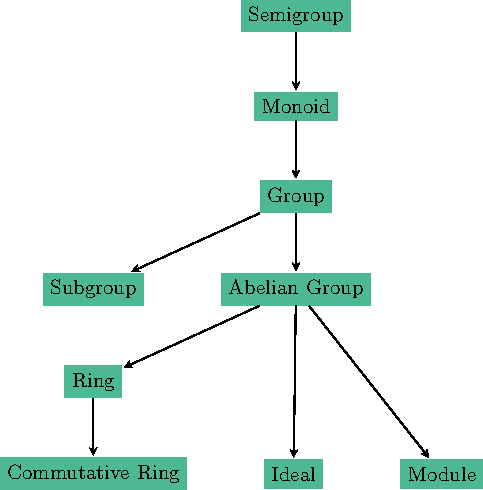
\includegraphics[width=.4\textwidth]{algebraic-structures.pdf}
\centering
\todo[inline]{To do:  Check source code to verify whether the hierarchy figure should be altered (subgroups/other subobjects, quotients, finitely generated modules, etc.)}
\end{figure}

We started by defining a semigroup class, which declares a binary operation to
be associative. From here, we build up through monoids, which introduce
identities, to groups, which introduce inverses. Note the double equals ``$==$'' in
these definitions is notation for an arbitrary equivalence relation over the
group's carrier set, which acts as equality.

\begin{minted}{coq}
  Infix "==" := equiv (at level 60, no associativity).
  Class Semigroup := {
    semigroup_assoc:
      forall (a b c: Carrier),
        a <o> b <o> c == a <o> (b <o> c);
  }.
  Class Monoid := {
    monoid_semigroup :> Semigroup equiv op;
    monoid_ident_l:
      forall (a: Carrier), ident <o> a == a;
    monoid_ident_r:
      forall (a: Carrier), a <o> ident == a;
  }.
  Class Group := {
    group_monoid :> Monoid equiv op ident;
    group_inv_l:
      forall (a: Carrier), inv a <o> a == ident;
    group_inv_r:
      forall (a: Carrier), a <o> inv a == ident;
  }.
\end{minted}
The lines of the form, e.g.,  ``\verb|monoid_semigroup :> Semigroup equiv op;|'' simply coerce
the monoid typeclass into a semigroup.

%While we found later on that we did not need quotients, 
While in the end, our formal proof did not call upon quotients of algebraic structures, quotient rings and quotient modules are fundamental to commutative algebra, and one can use them to construct alternate proofs of Nakayama's lemma.
It is worth pointing out that we have formalized quotients of algebraic objects  in Coq using typeclasses, which appear to work rather nicely. 

An algebraic quotient is, roughly, the set of equivalence classes of an algebraic structure with respect to an equivalence relation on its elements, for which the set of equivalence classes inherit the same kind of algebraic structure. 
For example, consider the quotient of a group modulo a subgroup, i.e. a subset of elements of the group that it itself a group under the group operations. 
Under equivalence relation on the group, every element of the subgroup must be in the same equivalence class as the identity.  
With \texttt{P} the predicate for the subgroup, there are two ways to
make an equivalence relation from this description.

\begin{minted}{coq}
  Definition left_congru (a b: Carrier) :=
    P (inv a <o> b).
  Definition right_congru (a b: Carrier) :=
    P (a <o> inv b).
\end{minted}
% \end{verbatim}
When these two relations coincide, then we can prove that this common equivalence
relation actually preserves the group structure. Subgroups which have this
property are called \emph{normal subgroups}.
% \begin{verbatim}
\begin{minted}{coq}
  Let normal_subgroup_congru_coincide :=
    forall (a b: Carrier),
      left_congru op inv P a b <->
      right_congru op inv P a b.

  Theorem quotient_normal_subgroup_group:
    normal_subgroup_congru_coincide ->
    Group (left_congru op inv P) op ident inv.
\end{minted}

The importance of quotients in commutative algebra motivates our use of equivalence relations to define the
components of a group structure. 
If one were to instead use the regular Leibniz equality,
it would be very difficult to identify a quotient group with another
group. 
However, by  defining a group in terms of an arbitrary equivalence relation, we enable our theory to state that a quotient group is
simply a group under a different equivalence. 
Not much is lost,  as Coq's setoid rewrite tactics can still be called upon; 
a setoid is a type equipped
with an equivalence relation.

Moving onward, we formalized the structure of a ring, which has two binary
operations:
addition, which must be commutative, and multiplication, which need not be commutative in general.
Next we defined the structure of a commutative ring, further requiring commutativity of multiplication, as well as a multiplicative identity. 
At this point,, we define {ideals} of commutative rings as normal subgroups of the ring under
addition that satisfy the absorption property under multiplication, i.e., \(r a\) is in
the ideal for every element \(a\) of the ideal, and every element \(r\) of the commutative ring.


Again, we defined quotient rings but found them unnecessary in the end. Note
that should an ideal \(I\) contain a unit, an element \(x\) with a
multiplicative inverse \(x^{-1}\), then \(I\) would be the entire ring by the
absorbing property: given any element \(a\) of the ring, then \(a x^{-1}\) is
also in the ring, and \(a x^{-1} x = a 1 = a\in I\). Maximal ideals were
defined next. These are ideals that are proper subsets of the ring while having
no larger ideal except for the ring itself. Below is the definition in Coq,
which uses \texttt{P} as the predicate for the ideal.
% \begin{verbatim}
\begin{minted}{coq}
  Definition maximal_ideal :=
    exists (r: Carrier), (not (P r) /\
      forall (Q: Carrier -> Prop)
          (Q_proper: Proper (equiv ==> iff) Q)
          (Q_ideal: Ideal add zero minus mul Q),
        (forall (r: Carrier), P r -> Q r) ->
        (forall (r: Carrier), Q r) \/
          (forall (r: Carrier), Q r -> P r)).
\end{minted}
% \end{verbatim}
Almost by definition, maximal ideals can contain no units, otherwise they would
fail to be a proper subset of the ring. We could then define a local ring,
which is a ring with a single maximal ideal.
% \begin{verbatim}
\begin{minted}{coq}
  Definition local_ring :=
    exists (P: Carrier -> Prop)
        (P_proper: Proper (equiv ==> iff) P)
        (P_ideal: Ideal add zero minus mul P),
      maximal_ideal P /\
      (forall (Q: Carrier -> Prop)
          (Q_proper: Proper (equiv ==> iff) Q)
          (Q_ideal: Ideal add zero minus mul Q),
        maximal_ideal Q -> forall (r: Carrier), P r <-> Q r).
\end{minted}
% \end{verbatim}

Here we had to include an axiom that in commutative ring, any non-unit \(x\) is
contained in some maximal ideal. This was made into an axiom as the standard
mathematical argument is a proof with potentially infinitely many steps. The
standard argument goes as follows.
\begin{quote}
    Set \(I_{1}\coloneqq (x)\) to be the principal ideal for \(x\), i.e. the
    ideal generated by the single element \(x\). If \(I_{1}\) is not maximal,
    then there exists a strictly larger ideal \(I_{2}\), i.e.
    \(x\in I_{1}\subsetneq I_{2}\). If \(I_{2}\) is not maximal, then there
    exists another strictly larger ideal \(I_{3}\). Continue these arguments
    infinitely many times if necessary in order to get an infinite chain of
    ideals containing \(x\).
    \[x\in I_{1}\subsetneq I_{2}\subsetneq I_{3}\subsetneq\cdots\subsetneq R\]
    It is a simple matter to show that \(\bigcup_{k=1}^{\infty} I_{k}\) is also
    an ideal containing in \(x\). So by Zorn's lemma, there exists a maximal
    ideal in \(R\) which contains \(x\).
\end{quote}
Zorn's lemma is equivalent to the axiom of choice. So we had to add at least
one axiom here in order to proceed. By adding the axiom that we did, not only
will we encapsulate an infinite argument, but we will also avoid the need for
the axiom of choice.

Also, we used classical logic to prove that \(1 - x\) is a unit where \(x\) is
a non-unit in any local ring. The proof used the rule \(\neg\neg P\rightarrow
P\) in order to do a proof by contradiction.

The next structure defined were modules over rings which generalize vector
spaces over fields. We needed to capture the notion of linear combinations of
coefficients and module vectors. This was done by dependently typed vectors,
i.e. lists parameterized by their length. Because there is an overload of the
term ``vector'', we will use that term to refer to module vectors, and use the
term ``list'' to mean length parameterized lists. As we don't use the simpler
kind of lists, this avoids any name collisions. A finitely generated module is
like the vector space \(\mathbf{R}^{n}\) in that there are finitely many
vectors which can generate all other vectors, for \(\mathbf{R}^{n}\) one such
collection of generators are \(\mathbf{e}_{1} = \begin{pmatrix} 1 & 0 & 0 &
  \cdots & 0\end{pmatrix}^{T}\), \(\mathbf{e}_{2} = \begin{pmatrix} 0 & 1 & 0 &
  \cdots & 0\end{pmatrix}^{T}\), \textellipsis, \(\mathbf{e}_{n} =
  \begin{pmatrix} 0 & 0 & 0 & \cdots & 1\end{pmatrix}^{T}\). In our code,
\texttt{M} is the type of module elements, \texttt{R} is the type of ring
elements which act as coefficients, and \texttt{t A n} is a list whose elements
are of type \texttt{A} and whose length is \texttt{n}.
% \begin{verbatim}
\begin{minted}{coq}
  Definition finitely_generated {n: nat}(basis: t M n) :=
    forall (vector: M),
      exists (coeffs: t R n),
        vector =M= linear_combin coeffs basis.
\end{minted}
% \end{verbatim}

Next, we defined the product of an ideal \(I\) and a module \(M\), denoted as
\(I M\), which is defined to be all linear combinations of vectors from \(M\)
and coefficients from \(I\). This can be easily shown to be a submodule of
\(M\). We represented this in Coq as a predicate over \(M\).
% \begin{verbatim}
\begin{minted}{coq}
  Context (P: R -> Prop).
  Context {P_proper: Proper (Requiv ==> iff) P}.
  Context {P_ideal: Ideal Radd Rzero Rminus Rmul P}.
  
  Definition ideal_module (x: M): Prop :=
    exists (n: nat)(coeffs: t R n)(vectors: t M n),
      Forall P coeffs /\
      x =M= linear_combin Madd Mzero action coeffs vectors.
\end{minted}
% \end{verbatim}
The \verb|Forall P coeffs| ensures that every element of the coefficient list
\texttt{coeffs} satisfies the predicate \texttt{P}. From here, we can move to
stating Nakayama's lemma.

\subsection{Formal Proof of Nakayama's Lemma}


\begin{theorem}[Nakayama's lemma]
  Let \(M\) be a finitely generated module over a local ring \(R\) with maximal
  ideal \(\mathfrak{m}\). If \(\mathfrak{m} M = M\), then \(M = 0\), which is
  to say that \(M\) is the zero module which consists of exactly one element,
  that being the zero vector.
\end{theorem}

We needed a lemma before moving on to prove the main theorem which states that
for a finitely generated module \(M\) with a basis
\(b_{1}, b_{2}, \dots, b_{n}\), any element \(x\in I M\) where \(I\) is an
ideal can be written as a linear combination of the basis vectors with
coefficients coming from \(I\). The proof of this lemma is straightforward and
follows the standard, informal mathematical argument which inductively goes
through the vectors needed to generate \(x\) and shows that each vector can be
rewritten in terms of the basis vectors times elements of the ideal \(I\) as
follows.
\begin{align*}
  x & = \sum_{k=1}^{m} u_{k} a_{k} \\
    & = \sum_{k=1}^{m} u_{k} (r_{k1} b_{1} + \cdots + r_{kn} b_{n}) \\
    & = \sum_{j=1}^{n} (u_{1} r_{1j} + \cdots + u_{m} r_{mj}) b_{j}
\end{align*}
Since each \(u_{k}\) comes from the ideal \(I\), the absorbing property of
ideals guarantees that \(u_{k} r_{k j}\) is also contained in \(I\). As ideals
are also closed under addition, it follows that \(u_{1} r_{1j} + \cdots +
u_{m} r_{m j}\) are all elements of \(I\). Thus, \(x\) can be written as a
linear combination of the basis vectors with the coefficients coming from
\(I\).

For the proof of Nakayama's lemma, it too follows the standard, informal
mathematical argument. Do induction on the number of vectors needed to generate
the module \(M\). The base case where \(M\) is generated by 0 vectors is by
definition true since an empty linear combination is conventionally taken to be
the zero vector. The inductive case where \(M\) is generated by the vectors
\(b_{1}, \dots, b_{m}, b_{m+1}\). By assumption \(M = \mathfrak{m} M\) with
\(b_{1}\in M\). Then \(b_{1}\in\mathfrak{m} M\) meaning that by our lemma,
there exists a linear combination for \(b_{1}\), say
\[b_{1} = u_{1} b_{1} + \cdots + u_{m+1} b_{m+1}\]
for some \(u_{1}, \dots, u_{m+1}\in\mathfrak{m}\). Collect the \(b_{1}\) terms
on the left-hand side of the equation to get that
\[(1 - u_{1}) b_{1} = u_{2} b_{2} + \cdots + u_{m+1} b_{m+1}\text{.}\]
As mentioned when defining maximal ideals, \(\mathfrak{m}\) can only contain
non-units. Namely, \(u_{1}\) must be a non-unit. Then we had already proven
that \(1 - u_{1}\) is a unit as we are in a local ring. Let \(v_{1}\) be the
multiplicative inverse of \(1 - u_{1}\), and multiply it on both sides of the
equation.
\begin{align*}
  v_{1} (1 - u_{1}) b_{1}
    & = v_{1} u_{2} b_{2} + \cdots + v_{1} u_{m+1} b_{m+1} \\
  1 b_{1} & = \\
  b_{1} & = v_{1} u_{2} b_{2} + \cdots + v_{1} u_{m+1} b_{m+1} \\
\end{align*}
We have thus found that one of the basis vectors is not needed to generate this
module. Using the induction hypothesis, we have that \(M = 0\). Showing that
the induction hypothesis holds in Coq takes more work than in an informal
proof, but this extra work is just a lot of bookkeeping.

\bibliographystyle{plain}
\bibliography{references}
\end{document}
